\documentclass[11pt]{article}

% Change "review" to "final" to generate the final (sometimes called camera-ready) version.
% Change to "preprint" to generate a non-anonymous version with page numbers.
\usepackage[review]{acl}

% Standard package includes
\usepackage{times}
\usepackage{latexsym}
\usepackage[table]{xcolor}
\usepackage{placeins}
\usepackage{tabularx}

% For proper rendering and hyphenation of words containing Latin characters (including in bib files)
\usepackage[T1]{fontenc}
% For Vietnamese characters
% \usepackage[T5]{fontenc}
% See https://www.latex-project.org/help/documentation/encguide.pdf for other character sets

% This assumes your files are encoded as UTF8
\usepackage[utf8]{inputenc}

% This is not strictly necessary, and may be commented out,
% but it will improve the layout of the manuscript,
% and will typically save some space.
\usepackage{microtype}

% This is also not strictly necessary, and may be commented out.
% However, it will improve the aesthetics of text in
% the typewriter font.
\usepackage{inconsolata}

%Including images in your LaTeX document requires adding
%additional package(s)
\usepackage{graphicx}
\usepackage{float}

% If the title and author information does not fit in the area allocated, uncomment the following
%
%\setlength\titlebox{<dim>}
%
% and set <dim> to something 5cm or larger.

\title{Dialogue-Semantic Grounding Failures in Zero-Shot Cross-Lingual Summarization with Small Language Models}

\author{
Yunwoo Lee, Jennifer Huang, Ziwa Li \\
Department of Linguistics, University of Washington, Seattle, WA, USA \\
\texttt{\{yunu919, jjnhuang, lizhihua\}@uw.edu}
}

\begin{document}
\maketitle
\begin{abstract}
Cross-lingual dialogue summarization with small language models (SLMs) can produce fluent but unfaithful target-language summaries. We study zero-shot English-to-Chinese dialogue summarization by comparing three open-weight SLMs with a supervised mBART baseline using ROUGE, BERTScore, OmniScore, and manual error analysis. We introduce a Dialogue-Semantic Grounding Error Taxonomy covering participants, events, speaker roles, circumstantial details, modality, discourse outcomes, omissions, and language issues. Although mBART achieves the strongest reference-based scores, it has the lowest manually determined no-error rate (20\%), compared with 63\% for the best-performing SLM. These results show that reference similarity and fluency can conceal systematic dialogue-grounding failures.
\end{abstract}

\section{Introduction}
Large language models (LLMs) achieve strong performance on generation tasks, including summarization, but their computational and deployment costs limit their use in resource-constrained, industrial, and privacy-sensitive settings \citep{abrougui-etal-2026-small,xu-etal-2025-evaluating}. Small language models (SLMs) offer a more efficient and locally deployable alternative, with recent work exploring their potential for resource-constrained summarization and cross-lingual transfer \citep{xu-etal-2025-evaluating,philippy-etal-2025-enhancing}. Yet it remains unclear whether SLMs can generate summaries that are not only fluent, but also faithfully grounded in the source input.

We study this question through zero-shot English-to-Chinese dialogue summarization. This setting is diagnostic because the model must understand the English dialogue, identify salient events and speaker roles, and express the result in Chinese \citep{wang-etal-2022-clidsum,wang-etal-2023-zero}. Previous studies have shown that cross-lingual summarization is sensitive to dataset construction, translation artifacts, and evaluation design \citep{bhattacharjee-etal-2023-crosssum,wang-etal-2023-understanding}. However, automatic metrics and final-summary evaluation alone may obscure how outputs fail to preserve dialogue meaning.

This paper provides a diagnostic analysis. We compare open-weight SLMs with an mBART baseline using ROUGE, BERTScore, and OmniScore, and then conduct a fine-grained error analysis. To connect hallucination analysis with dialogue semantics, we develop a Dialogue-Semantic Grounding Error Taxonomy. Inspired by work showing that conversational understanding requires tracking participants, actions, semantic roles, references, and context across turns \citep{aghajanyan-etal-2020-conversational}, our taxonomy distinguishes errors involving entities, events, speaker roles, circumstantial details, modality, discourse outcomes, omissions, and language or format issues. Our analysis shows that hallucinations in zero-shot cross-lingual dialogue summarization are not only surface-level generation errors, but often reflect breakdowns in dialogue-semantic grounding across languages.

\section{Experimental Setup}
\subsection{Data}

We evaluate models on XSAMSum, the dialogue summarization dataset released as part of the ClidSum benchmark \citep{wang-etal-2022-clidsum}. XSAMSum extends the English SAMSum corpus \citep{gliwa-etal-2019-samsum} to a cross-lingual setting by pairing English messenger-style dialogues with professional summaries in multiple target languages. We focus on English-to-Chinese summarization, where the input is an English dialogue and the reference output is a Chinese summary.

For diagnostic evaluation, we use a fixed random sample of 100 test examples selected with seed 42 from the XSAMSum test split. All models are evaluated on the same examples to support paired comparison across systems. We apply minimal preprocessing, formatting each dialogue as speaker-prefixed turns separated by newline characters, following the original ClidSum setup.


\subsection{Models}

We evaluate one fine-tuned sequence-to-sequence baseline and three open-weight instruction-tuned small language models (SLMs). As a supervised baseline, we use mBART-large-50 fine-tuned for English-to-Chinese dialogue summarization. The model is trained with a maximum input length of 768 tokens, a maximum target length of 64 tokens, 5 epochs, a learning rate of $2\times10^{-5}$, and an effective batch size of 24. During evaluation, we decode with beam search using 5 beams.

For zero-shot evaluation, we select open-weight instruction-tuned models with fewer than 10B parameters: Aya Expanse 8B, Gemma 4 E4B, and Qwen 3.5 9B. We refer to these models as SLMs in a deployment-oriented sense, since they are substantially smaller than frontier-scale LLMs and can be run locally using quantized checkpoints. All three SLMs are evaluated in the same zero-shot direct setting: given an English dialogue, each model is prompted to generate a concise Simplified Chinese summary directly, without demonstrations, intermediate translation, or task-specific fine-tuning. We use the same prompt for all three models; the full template is provided in Appendix~\ref{sec:appendix-inference}.

\subsection{Evaluation}

We evaluate model outputs using three complementary approaches: reference-based automatic metrics, LLM-based evaluation, and dialogue-semantic grounding error analysis.

\paragraph{Reference-based metrics.}
We compute ROUGE \citep{lin-2004-rouge} and BERTScore \citep{zhang2020bertscoreevaluatingtextgeneration} against the Chinese reference summaries. ROUGE measures lexical overlap between the generated and reference summaries, while BERTScore provides a contextual embedding-based estimate of semantic similarity. These metrics provide aggregate reference-based signals, but they do not directly identify which aspects of the dialogue meaning are preserved or distorted.

\paragraph{LLM-based evaluation.}
We additionally use the reference-based OmniScore \citep{alam-etal-2026-omniscore} as a learned evaluation metric for summary quality and faithfulness. OmniScore evaluates each generated summary relative to the Chinese reference along four dimensions: informativeness, clarity, plausibility, and faithfulness. It provides a complementary signal to ROUGE and BERTScore, especially when lexical overlap is limited by cross-lingual generation.

\paragraph{Dialogue-semantic grounding error analysis.}
To diagnose failure modes not captured by aggregate scores, we manually annotate generated summaries using the Dialogue-Semantic Grounding Error Taxonomy shown in Table~\ref{tab:taxonomy}. This approach follows fine-grained summarization evaluation work that decomposes summary quality into factuality and key-information alignment \citep{song-etal-2024-finesure}. Our taxonomy adapts this diagnostic perspective to English-to-Chinese dialogue summarization by targeting whether participants, events, roles, and discourse relations are preserved across languages.

\begin{table}[t]
\centering
\footnotesize
\setlength{\tabcolsep}{3pt}
\begin{tabularx}{\columnwidth}{@{}lX@{}}
\hline
Label & Definition \\
\hline
\textsc{H-Ent}  & Incorrect or unsupported participant, entity, name, or object. \\
\textsc{H-Evt}  & Incorrect, altered, or unsupported event or action. \\
\textsc{H-Role} & Incorrect speaker attribution or participant role. \\
\textsc{H-Circ} & Incorrect time, place, number, quantity, or condition. \\
\textsc{H-Mod}  & Incorrect negation, modality, intention, or uncertainty. \\
\textsc{H-Disc} & Incorrect discourse relation, decision, agreement, or outcome. \\
\textsc{Omit}   & Omission of salient information needed to understand the dialogue. \\
\textsc{Lang}   & Language, translation, formatting, or instruction-following issue. \\
\textsc{No-Error} & No identified grounding or language error. \\
\hline
\end{tabularx}
\caption{Dialogue-Semantic Grounding Error Taxonomy. Hallucination labels are prefixed with \textsc{H-}.}
\label{tab:taxonomy}
\end{table}

For each model output, we compare the generated Chinese summary with the English source dialogue and assign one or more labels corresponding to the errors present. Outputs without an identified grounding or language problem are labeled \textsc{No-Error}. Because multiple grounding failures may occur in the same summary, the error categories are not mutually exclusive.

\FloatBarrier

\section{Results}

\begin{table*}[!t]
\centering
\small
\begin{tabular}{lrrrrrrrrr}
\hline
Model & R-1 & R-2 & R-L & BERTScore & Info. & Clar. & Plaus. & Faith. & Len. \\
\hline
Aya Expanse 8B & 26.53 & 7.89 & 20.84 & 70.11 & 3.26 & 4.02 & 4.04 & \textbf{3.17} & 3.52 \\
Gemma 4 E4B    & 30.27 & 8.32 & 23.68 & 70.85 & 3.17 & 3.95 & 4.00 & 2.96 & 2.40 \\
Qwen 3.5 9B    & 28.35 & 7.62 & 22.42 & 70.47 & 3.22 & 3.88 & 3.97 & 3.00 & 2.89 \\
mBART-large    & \textbf{41.95} & \textbf{18.10} & \textbf{34.85} &
\textbf{77.64} & 2.97 & \textbf{4.24} & \textbf{4.17} & 2.92 & 1.03 \\
\hline
\end{tabular}
\caption{Mean reference-based evaluation scores and generated-to-reference length ratios. OmniScore dimensions are reported on their original scale. Bold indicates the highest value in each quality metric; length ratio is descriptive and is not ranked.}
\label{tab:automatic-results}
\end{table*}

\subsection{Automatic Evaluation}

Table~\ref{tab:automatic-results} presents the reference-based evaluation results. The supervised mBART baseline obtained the highest ROUGE and BERTScore values, with ROUGE-1 of 41.95 and BERTScore of 77.64. Among the zero-shot SLMs, Gemma achieved the highest ROUGE scores and BERTScore, although the differences among the three SLMs were relatively small.

The reference-based OmniScore dimensions showed a less uniform pattern. mBART received the highest clarity (4.24) and plausibility (4.17) scores but the lowest faithfulness score (2.92). Aya obtained the highest faithfulness score (3.17), followed by Qwen (3.00) and Gemma (2.96).

Output length differed substantially across systems. The mean generated-to-reference length ratio was 1.03 for mBART, compared with 2.40 for Gemma, 2.89 for Qwen, and 3.52 for Aya. Thus, the zero-shot SLM summaries were generally substantially longer than the Chinese references, whereas mBART produced outputs of approximately reference length.

\begin{table}[H]
\centering
\small
\begin{tabular}{lrrrr}
\hline
Model & No err. & Halluc. & Omit & Lang. \\
\hline
Aya Expanse & 38 & 43 & 7 & 17 \\
Gemma       & \textbf{63} & \textbf{29} & 8 & \textbf{0} \\
Qwen        & 58 & 39 & \textbf{3} & \textbf{0} \\
mBART       & 20 & 61 & 48 & 11 \\
\hline
\end{tabular}
\caption{Percentage of outputs assigned to aggregated grounding-error categories. \textit{Halluc.} denotes any \textsc{H-*} label. Categories may overlap when an output contains multiple errors.}
\label{tab:grounding-results}
\end{table}

\subsection{Dialogue-Semantic Grounding Errors}

The manual grounding analysis produced a markedly different system ranking from the reference-based metrics. As shown in Table~\ref{tab:grounding-results}, Gemma had the highest rate of outputs with no identified error (63\%), followed by Qwen (58\%), Aya (38\%), and mBART (20\%). Conversely, mBART had the highest rate of hallucination errors (61\%) and omissions (48\%). Gemma had the lowest hallucination rate (29\%), while Qwen had the lowest omission rate (3\%).

The fine-grained labels also revealed model-specific error profiles. Speaker-role errors were the most frequent hallucination type for Aya (21\%) and were also common for Qwen (14\%). For mBART, event hallucinations were especially frequent (32\%), followed by speaker-role errors (21\%), entity errors (16\%), and circumstantial errors (16\%). Language or formatting problems occurred in 17\% of Aya outputs and 11\% of mBART outputs, but were not observed for Gemma or Qwen. Full label rates and paired comparisons are provided in Appendix~\ref{sec:appendix-diagnostics}.

Paired comparisons on the same 100 dialogues further supported these differences. Gemma produced an error-free output while mBART produced an erroneous output on 50 dialogues; the reverse pattern occurred on only 7 dialogues. Qwen had more paired wins than mBART (42 vs.\ 4), as did Aya (28 vs.\ 10). Gemma also had more paired wins than Aya (40 vs.\ 15) and Qwen (21 vs.\ 16).

Difficulty was shared across systems for a subset of the data. None of the four systems produced an error-free summary for 13 of the 100 dialogues, whereas all four systems succeeded on only four dialogues. These results indicate that some source dialogues consistently presented grounding difficulties across both supervised and zero-shot systems.

\FloatBarrier

\subsection{Divergence between Automatic Metrics and Grounding Judgments}

The automatic metrics did not consistently distinguish grounded from erroneous summaries. Using global quartiles across all 400 outputs, we treat the upper quartile of each metric as a descriptive high-score threshold. mBART produced 29 outputs that combined high mean ROUGE with a manually identified error and 34 that combined high BERTScore with an error. Conversely, the SLMs produced error-free summaries despite low reference overlap: 46 SLM outputs combined a lower-quartile mean ROUGE score with no identified error, and 39 combined a lower-quartile BERTScore with no error.

A similar mismatch occurred for reference-based OmniScore faithfulness. Twenty-five Aya outputs, 6 Gemma outputs, 9 Qwen outputs, and 13 mBART outputs received upper-quartile faithfulness scores despite containing a manually identified grounding error. Thus, even learned reference-based evaluation did not fully capture errors involving speaker roles, events, modality, or discourse outcomes.

The contrast was particularly pronounced for mBART: it ranked first on ROUGE, BERTScore, clarity, and plausibility, but last on the manually determined no-error rate. Among the zero-shot SLMs, Aya received the highest mean OmniScore faithfulness score, while Gemma achieved the highest manually determined no-error rate.

\subsection{Output Length and Error Structure}

Output length was associated most strongly with omission. Across all model outputs, length ratio was negatively correlated with omission ($\rho=-0.423$) and event hallucination ($\rho=-0.192$), while it was positively correlated with the absence of an identified error ($\rho=0.170$). Among summaries shorter than 75\% of the reference length, 65\% contained an omission. This rate decreased to 1.5\% among summaries more than four times the reference length. These aggregate relationships should be interpreted descriptively because output-length distributions differed substantially by model.

Grounding errors also frequently co-occurred. Seventy-six of the 400 outputs (19\%) received multiple labels. The most common combinations were event hallucination with omission (19 outputs), event hallucination with speaker-role error (11), and event hallucination with circumstantial error (10). This concentration of event-related combinations shows that erroneous summaries often contained interacting grounding failures rather than a single isolated error.

\FloatBarrier

\section{Discussion}

\subsection{Reference Similarity Does Not Guarantee Dialogue Grounding}

Our results reveal a substantial disconnect between reference-based evaluation and dialogue-semantic grounding. mBART achieved the highest ROUGE, BERTScore, clarity, and plausibility scores, yet had the lowest manually determined no-error rate and the highest rates of hallucination and omission. Conversely, the zero-shot SLMs sometimes produced grounded summaries despite receiving low ROUGE or BERTScore values. These cases suggest that similarity to a single reference summary does not reliably determine whether a generated summary preserves the meaning of the source dialogue.

One explanation is that the reference summary represents only one valid selection and formulation of the dialogue content. Because the SLM outputs were substantially longer, they could include supported dialogue details absent from the concise reference, reducing lexical overlap without necessarily introducing an error. In contrast, mBART generated outputs close to the reference length and achieved high reference overlap, but this did not prevent the omission or distortion of dialogue information. This result is especially relevant to cross-lingual summarization, where variation in content selection and target-language realization can further weaken the connection between reference overlap and source grounding.

The mismatch observed for OmniScore faithfulness points to a related limitation. In our setting, OmniScore evaluates faithfulness relative to the Chinese reference rather than directly against the English dialogue. It can therefore reward reference consistency without detecting whether participant roles, events, modality, or conversational outcomes have been misrepresented. Reference-based learned metrics remain useful indicators of summary quality, but our results suggest that they should be complemented by evaluation grounded directly in the source dialogue.

\subsection{Models Exhibit Distinct Grounding Trade-offs}

The results do not support a simple distinction in which supervised models are consistently more reliable than zero-shot SLMs, or vice versa. Instead, each system exhibited a distinct error profile. Gemma achieved the highest no-error rate and the lowest hallucination rate, whereas Qwen produced the fewest omissions. Aya received the highest reference-based OmniScore faithfulness score but showed more speaker-role and language-related errors. These differences indicate that aggregate quality scores can conceal substantially different grounding behavior among similarly sized instruction-tuned models.

mBART exhibited a different trade-off. Its outputs were concise, fluent, and similar to the references, but frequently omitted salient information or introduced event-level errors. Its high omission rate may be associated with its compressed generation behavior and supervised preference for short reference-style summaries, although the current analysis does not establish a causal relationship. By contrast, the SLMs generated considerably longer outputs, potentially preserving more dialogue content while also creating more opportunities for unsupported details or incorrect role assignments.

The association between output length and omission should therefore be interpreted cautiously. Shorter outputs were strongly associated with omission, but length distributions also differed systematically across models. Length may reflect broader differences in model architecture, training objectives, prompting, and decoding rather than independently determining grounding quality. Controlled generation experiments would be required to separate the effect of summary length from these system-level differences.

\subsection{Grounding Failures Are Structurally Related}

The fine-grained taxonomy shows that hallucinations were not limited to isolated entity substitutions or surface translation errors. Speaker-role, event, circumstantial, modality, and discourse-outcome errors directly affected the representation of who did what, under which conditions, and with what conversational result. Event errors also frequently co-occurred with omissions, role errors, and circumstantial errors. Such co-occurrence suggests that multiple summary errors can arise from a shared failure to construct or preserve the underlying dialogue situation.

This observation supports treating cross-lingual dialogue summarization as a grounding problem rather than only a translation or generation problem. A model must track participants across turns, attribute actions and statements to the correct speaker, distinguish asserted events from possibilities or negations, and preserve decisions and outcomes before expressing them in another language. Fluent Chinese generation can conceal failures at any of these intermediate levels.

The shared difficult examples provide further evidence that some challenges arise from the dialogues themselves rather than from a single model. Thirteen dialogues produced errors across all four systems, whereas only four were summarized without error by every system. Dialogues involving multiple speakers, shifting roles, implicit relations, or disputed outcomes may impose particular grounding demands. A more detailed analysis of these shared failures could help identify which dialogue structures are most challenging for cross-lingual summarization systems.


\section{Conclusion}

We presented a diagnostic analysis of zero-shot English-to-Chinese dialogue summarization with small language models. Reference-based metrics did not consistently reflect dialogue grounding: fluent, high-scoring summaries could still contain errors involving events, speaker roles, modality, discourse outcomes, and omissions. Our findings highlight the need to complement aggregate metrics with source-grounded, fine-grained evaluation when assessing cross-lingual summarization systems.

\section{Limitations}

Our study is limited to 100 English-to-Chinese dialogues, three zero-shot SLMs, and one supervised baseline, so the findings may not generalize to other languages, domains, prompts, or model families. The error analysis relies on manual judgments and may therefore be sensitive to annotator interpretation, while OmniScore is reference-based rather than directly grounded in the source dialogue. Finally, relationships involving output length are observational and may be confounded by model-specific generation behavior.



\bibliography{custom}

\clearpage
\appendix

\section{Detailed Diagnostic Results}
\label{sec:appendix-diagnostics}

\subsection{Zero-Shot Prompt and Inference Configuration}
\label{sec:appendix-inference}

All SLMs were run locally through Ollama using the same prompt template. The placeholder \texttt{\{dialogue\}} was replaced with the speaker-prefixed English dialogue without further task demonstrations. We used a temperature of 0.2, an 8,192-token context window, a maximum of 1,024 generated tokens, and disabled explicit reasoning output. The Ollama model identifiers were \texttt{aya-expanse:8b}, \texttt{gemma4:e4b}, and \texttt{qwen3.5:9b}.

\begin{center}
\fbox{%
\begin{minipage}{0.92\columnwidth}
\small\ttfamily\raggedright
You are an expert English-Chinese bilingual speaker. Given an English dialogue, please write a concise Simplified Chinese summary. Output only the summary, without titles or markdown.

\medskip
English dialogue:\par
\{dialogue\}

\medskip
Chinese summary:
\end{minipage}%
}
\end{center}

\noindent\textit{Prompt template used for all three SLMs.}

\subsection{Fine-Grained Error Profiles}

Figure~\ref{fig:model-label-rates} reports the rate of each taxonomy label among the 100 outputs produced by each model. Figure~\ref{fig:pairwise-wins} presents paired no-error wins; each cell indicates the number of dialogues for which the row model produced a \textsc{No-Error} output while the column model produced an output with at least one error.

\begin{figure}[!htbp]
\centering
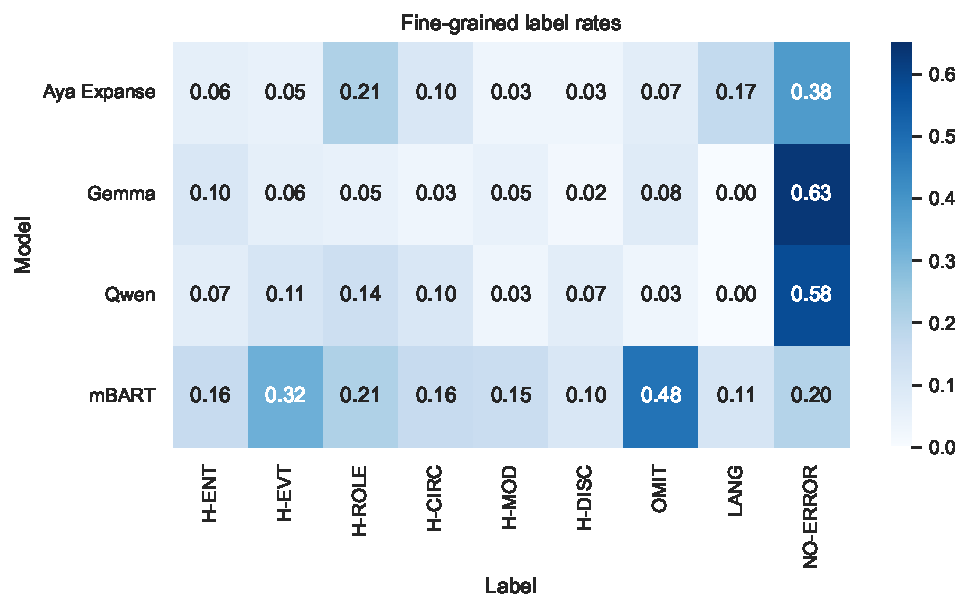
\includegraphics[width=\columnwidth]{figures/appendix/model_label_rates.pdf}
\caption{Fine-grained taxonomy-label rates by model. Each cell reports the proportion of a model's 100 outputs assigned the corresponding label.}
\label{fig:model-label-rates}
\end{figure}

\begin{figure}[!htbp]
\centering
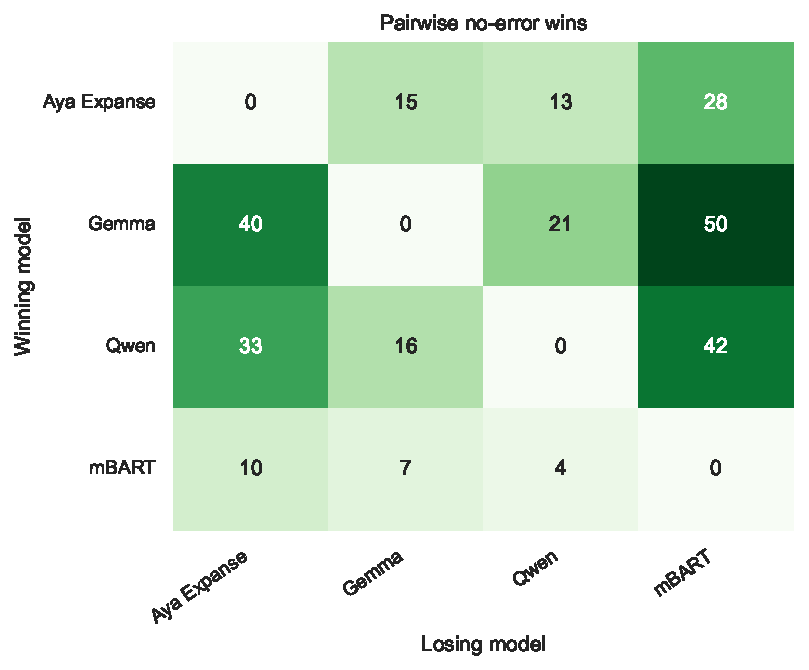
\includegraphics[width=0.95\columnwidth]{figures/appendix/pairwise_no_error_wins.pdf}
\caption{Paired \textsc{No-Error} wins. Rows represent winning models and columns represent losing models.}
\label{fig:pairwise-wins}
\end{figure}

\subsection{Sample-Level Difficulty}

Table~\ref{tab:appendix-difficulty} groups the 100 dialogues by the number of models that produced a \textsc{No-Error} output. Thirteen dialogues resulted in errors for all four systems, while only four were summarized without error by every system.

\begin{table}[!htbp]
\centering
\small
\begin{tabular}{rrr}
\hline
No-error models & Error models & Dialogues \\
\hline
0 & 4 & 13 \\
1 & 3 & 28 \\
2 & 2 & 30 \\
3 & 1 & 25 \\
4 & 0 & 4 \\
\hline
\end{tabular}
\caption{Sample-difficulty distribution based on the number of models producing a \textsc{No-Error} output.}
\label{tab:appendix-difficulty}
\end{table}

\subsection{Automatic-Metric and Annotation Mismatches}

Figure~\ref{fig:metric-mismatches} presents the distribution of automatic-metric mismatches. Mismatches are defined using global quartiles calculated across all 400 outputs. A high-score mismatch combines an upper-quartile metric score with at least one manually identified error. A low-score mismatch combines a lower-quartile score with a \textsc{No-Error} annotation.

\begin{figure}[!htbp]
\centering
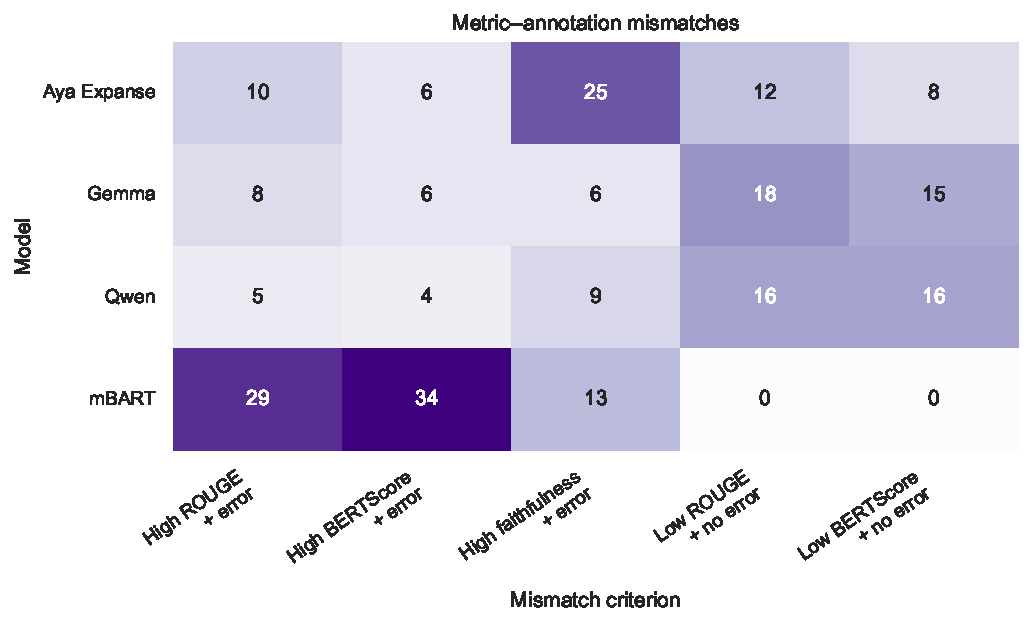
\includegraphics[width=\columnwidth]{figures/appendix/metric_annotation_mismatches.pdf}
\caption{Metric--annotation mismatch counts by model. High and low scores correspond to the global quartile thresholds in Table~\ref{tab:appendix-thresholds}.}
\label{fig:metric-mismatches}
\end{figure}

\begin{table}[!htbp]
\centering
\small
\begin{tabular}{lrr}
\hline
Metric & Lower quartile & Upper quartile \\
\hline
Mean ROUGE & 14.172 & 26.998 \\
BERTScore & 68.088 & 75.248 \\
OmniScore faithfulness & 2.692 & 3.296 \\
\hline
\end{tabular}
\caption{Global thresholds used to identify metric--annotation mismatches. Mean ROUGE is the arithmetic mean of ROUGE-1, ROUGE-2, and ROUGE-L.}
\label{tab:appendix-thresholds}
\end{table}

\subsection{Output Length and Error Labels}

Figure~\ref{fig:length-label-rates} reports label rates within generated-to-reference length-ratio bins. Table~\ref{tab:appendix-length-correlation} reports exploratory Spearman correlations between length ratio and each binary taxonomy-label indicator. The pooled relationships are descriptive because length distributions differ systematically across models.

\begin{figure}[!htbp]
\centering

\includegraphics[width=\columnwidth]{figures/appendix/length_label_rates.pdf}
\caption{Taxonomy-label rates within generated-to-reference length-ratio bins. Rates may overlap because outputs can receive multiple labels.}
\label{fig:length-label-rates}
\end{figure}

\begin{table}[!htbp]
\centering
\small
\begin{tabular}{lrr}
\hline
Label & $\rho$ & Labeled outputs \\
\hline
\textsc{No-Error} &  0.170 & 179 \\
\textsc{H-Role}   &  0.040 & 61 \\
\textsc{Lang}     &  0.027 & 28 \\
\textsc{H-Disc}   & -0.008 & 22 \\
\textsc{H-Ent}    & -0.038 & 39 \\
\textsc{H-Circ}   & -0.116 & 39 \\
\textsc{H-Mod}    & -0.127 & 26 \\
\textsc{H-Evt}    & -0.192 & 54 \\
\textsc{Omit}     & -0.423 & 66 \\
\hline
\end{tabular}
\caption{Spearman correlations between length ratio and binary taxonomy-label indicators across all 400 outputs.}
\label{tab:appendix-length-correlation}
\end{table}

\subsection{Multi-Label Error Co-Occurrence}

Seventy-six outputs received more than one error label. Figure~\ref{fig:multilabel-cooccurrence} presents the complete co-occurrence matrix, while Table~\ref{tab:appendix-cooccurrence} lists the most frequent combinations.

\begin{figure}[!htbp]
\centering

\includegraphics[width=\columnwidth]{figures/appendix/multilabel_cooccurrence.pdf}
\caption{Pairwise co-occurrence counts among error labels in the 76 multi-label outputs.}
\label{fig:multilabel-cooccurrence}
\end{figure}

\begin{table}[!htbp]
\centering
\small
\begin{tabular}{llr}
\hline
Label 1 & Label 2 & Count \\
\hline
\textsc{H-Evt}  & \textsc{Omit}   & 19 \\
\textsc{H-Evt}  & \textsc{H-Role} & 11 \\
\textsc{H-Circ} & \textsc{H-Evt}  & 10 \\
\textsc{H-Circ} & \textsc{Omit}   & 9 \\
\textsc{H-Ent}  & \textsc{H-Role} & 8 \\
\textsc{H-Role} & \textsc{Omit}   & 8 \\
\textsc{H-Evt}  & \textsc{H-Mod}  & 8 \\
\textsc{H-Ent}  & \textsc{H-Evt}  & 8 \\
\textsc{H-Ent}  & \textsc{Omit}   & 8 \\
\textsc{Lang}   & \textsc{Omit}   & 7 \\
\hline
\end{tabular}
\caption{Ten most frequent error-label combinations.}
\label{tab:appendix-cooccurrence}
\end{table}

\end{document}
